%%%%%%%%%%%%%%%%%%%% author.tex 
%%%%%%%%%%%%%%%%%%%%%%%%%%%%%%%%%%%
%
% sample root file for your "contribution" to a proceedings volume
%
% Use this file as a template for your own input.
%
%%%%%%%%%%%%%%%% Springer 
%%%%%%%%%%%%%%%%%%%%%%%%%%%%%%%%%%


\documentclass{svproc}
%
% RECOMMENDED 
%%%%%%%%%%%%%%%%%%%%%%%%%%%%%%%%%%%%%%%%%%%%%%%%
%%%
%
\usepackage{graphicx}
\usepackage{marvosym}
\usepackage{amsmath}
\usepackage{amssymb}
\usepackage{cite}

%\usepackage[russian]{babel}

% to typeset URLs, URIs, and DOIs
\usepackage{url}
\usepackage{hyperref}
\def\UrlFont{\rmfamily}

\def\orcidID#1{\unskip$^{[#1]}$}
\def\letter{$^{\textrm{(\Letter)}}$}

\begin{document}
\mainmatter              % start of a contribution
%
\title{Parallel Global Search Algorithm for Optimization of the Kinetic Parameters of Chemical Reactions}
%
\titlerunning{Parallel Global Search}  % abbreviated title (for running head)
%                                     also used for the TOC unless
%                                     \toctitle is used
%
\author{
Irek Gubaydullin$^{1,2}$\and
Leniza Enikeeva$^{2,3}$\orcidID{0000-0003-4219-4870}
\and
Konstantin Barkalov$^4$\orcidID{0000-0001-5273-2471}
\and
Ilya Lebedev$^4$\orcidID{0000-0002-8736-0652} 
}

%
\authorrunning{I. Gubaydullin et al.} % abbreviated author list (for running head)
%
%%%% list of authors for the TOC (use if author list has to be modified)
%\tocauthor{Konstantin Barkalov and Ilya Lebedev }
%

\institute{$^1$Institute of Petrochemistry and Catalysis – Subdivision of the Ufa Federal Research Centre of RAS, Ufa, Russia\\$^2$Ufa State Petroleum Technological University, Ufa, Russia \\$^3$Novosibirsk State University, Novosibirsk, Russia\\$^4$Lobachevsky State University of Nizhny Novgorod, Nizhny Novgorod, Russia\\
\email{leniza.enikeeva@yandex.ru},
\email{konstantin.barkalov@itmm.unn.ru},
\email{ilya.lebedev@itmm.unn.ru}
}

	
\maketitle              % typeset the title of the contribution

\begin{abstract}
The paper considers the application of parallel computing technology to the simulation of a catalytic chemical reaction, which is widely used in the modern chemical industry to produce synthesis gas. As a chemical reaction, the process of pre-reforming propane on a Ni catalyst is assumed. To simulate a chemical process, it is necessary to develop a kinetic model of the process, that is, to determine the kinetic parameters. To do this, the inverse problem of chemical kinetics is solved, which predicts the values of kinetic parameters based on laboratory data. From a mathematical point of view, the inverse problem of chemical kinetics is a global optimization problem. A parallel information-statistical global search algorithm was used to solve it. The use of the parallel algorithm has significantly reduced the search time to find the optimum. The found optimal parameters of the model made it possible to adequately simulate the process of pre-reforming propane on a Ni-catalyst.

\keywords{Global optimization $\cdot$ Multiextremal functions $\cdot$ Parallel computing $\cdot$ Chemical kinetics $\cdot$ Inverse problems }
\end{abstract}

\section{Introduction}

%Одним из направлений лаборатории математической химии Института нефтехимии и катализа УФИЦ РАН является исследование химических реакций методами математического моделирования. На данный момент изучено большое количество сложных химических процессов -- реакция циклоалюминирования алкенов триэтилалюминием в алюмациклопентаны, реакция гидроалюминирования олефинов алюминийорганическими соединениями, реакция спиртов с диметилкарбонатом и др. Математическое описание химических реакций необходимо для построения математических моделей химической кинетики, которые называются кинетическими моделями. Кинетическая модель является основой математического моделирования химических реакций и исходным уровнем при математическом моделировании химических реакторов. При разработке кинетической модели многостадийной химической реакции решается обратная задача химической кинетики (ХК). Обратной задачей ХК в общем случае называют процесс выбора механизма сложного процесса и определение его количественных характеристик -- констант скорости одностадийных реакций на основе опытных данных о динамике протекания процесса. С математической точки зрения обратная задача химической кинетики представляет собой задачу оптимизации, поэтому актуальной является задача выбора метода оптимизации. 

One of the areas of the Laboratory of Mathematical Chemistry of the Institute of Petrochemistry and Catalysis of the UFIC RAS is the study of chemical reactions by mathematical modeling methods. At the moment, a large number of complex chemical processes have been studied, among  them, the reaction of cycloalumination of alkenes with triethylaluminium into alumacyclopentanes, the reaction of hydroalumination of olefins with organoaluminum compounds, the reaction of alcohols with dimethyl carbonate, etc. The mathematical description of chemical reactions is necessary for the development the mathematical models of chemical kinetics, which are called kinetic models. The kinetic model is the basis for mathematical modeling of chemical reactions and the initial level for mathematical modeling of chemical reactors. When developing a kinetic model of a multi-stage chemical reaction, the inverse problem of chemical kinetics (CK) is solved. The inverse problem of CK is generally called the process of selecting the mechanism of a complex process and determining its quantitative characteristics -- the rate constants of reactions based on experimental data about the dynamics of the process. From a mathematical point of view, the inverse problem of chemical kinetics is a global optimization problem, so the problem of choosing an optimization method is relevant.


%Метод решения оптимизационных задач подобного типа должен учитывать следующую специфику. Во-первых, целевая функция задачи является "черным ящиком", т.к. она задается не в виде формулы, а в виде некоторого алгоритма вычисления ее значений. Во-вторых, вычисление даже одного значения целевой функции является трудоемкой операцией, т.к. требует численного моделирования. Перечисленная специфика не позволяет задействовать для решения обратных задач мультистартовые методы, основанные на идеях многократного градиентного спуска. С одной стороны, вычисление градиента в данном случае будет чрезмерно дорогой операцией, а с другой стороны - мультистартовые методы слабо применимы для существенно многоэкстремальных задач, какими и являются обратные задачи химической кинетики. Перечисленные особенности inverse problem of chemical kinetics учитываются в разработанном в University of Nizhni Novgorod параллельном алгоритме глобальной оптимизации. Теоретическим базисом данного алгоритма является information-statistical approach, детально изложенный в \cite{Strongin2000}. Разработанный алгоритм основан на редукции исходной многомерной задачи к эквивалентной ей одномерной задаче с последующим ее решением эффективными методами оптимизации функций одной переменной. Вопросы распараллеливания алгоритма на разных архитектурах рассмотрены в \cite{Barkalov2016}. В данной статье представлены результаты, полученные при использовании parallel global search algorithm для решения inverse problem of chemical kinetics.

A method for solving the optimization problems of such type should account for the following aspects. First, the objective function of the problem is a ``black box'' since it is defined not by a formula but in the form of some algorithm for computing its values. Second, computing even a single value of the objective function is time-consuming operation since it requires numerical modeling \cite{Modorskii2016}. The aspects listed above don't allow employing the multistart methods based on the ideas of multiple gradient descents for solving the inverse problems. On one hand, computing the gradients would be too expensive operation in this case. On the other hand, the multistart methods are hardly applicable for the essentially multiextremal problems, which the inverse problems of chemical kinetics belong to.

The features of inverse problems of chemical kinetics listed above were taken into account in the parallel global search algorithm developed in University of Nizhni Novgorod. The information-statistical approach described in \cite{Strongin2000} in details makes a theoretical basis for this algorithm. The developed algorithm is based on a reduction of the initial multidimensional problem to an equivalent one-dimensional problem followed by solving the latter by efficient optimization methods for the functions of single variable. The issues of the parallelization of the algorithm on various architectures were considered in \cite{Barkalov2016,Strongin2018,Barkalov2020}. In the present paper, the results obtained with the use of the parallel global search algorithm for solving the inverse problem of chemical kinetics are presented.



\section{Mathematical Model}\label{Sec_math_mod}

The process under study is propane pre-reforming into methane-rich gas over Ni catalyst, which is an industrially important chemical process \cite{USKOV2019126741, Uskov_en}. Pre-reforming of propane was studied over industrial nickel-chromium catalyst at pressure of 1 and 5 bar in the temperature range of 220 -- 380 $^0$C and at flow rates of 4000 and 12000 h$^{-1}$. The experimental data on propane pre-reforming was acquired from our previous work \cite{Uskov_en}.  The reaction scheme consists of two reactions: propane steam conversion and CO$_2$ methanation \cite{Uskov_cat}:
\begin{gather}
C_3H_8 + 6H_2O \rightarrow 10H_2 + 3CO_2 \label{reac_ref}\\
CO_2 + 4H_2 \rightleftharpoons CH_4 + 2H_2O \label{reac_met},
\end{gather}
where the rates of reactions \eqref{reac_ref} -- \eqref{reac_met} are expressed according to the Langmuir-Hinshelwood model \cite{USKOV2019126741}:

\[
W_{ref} = \dfrac{k_{ref}^0 \cdot \exp \left(- \dfrac{E_{ref}}{RT} \right) }{\left(1 + B \cdot C_{C3H8}\right)^m},
\]

\[
W_{met} = k_{met}^0 \cdot \exp \left(- \dfrac{E_{met}}{RT} \right) \cdot C_{H2} \cdot \left[1 - \dfrac{P_{CH4} P_{H2O}^2}{K_{eq} P_{CO2} P_{H2}^4 }\right] ,
\]
where $W_{ref}$ and $W_{met}$ are the reaction rates; $E_{ref}$ and $E_{met}$ are the observed activation energies, J/mol; $k^0_{ref}$ and $k^0_{met}$ are the pre–exponential multipliers; $B$ is the constant parameter, $T$ is the temperature, K; $R$ is the universal gas constant, J/(K$\cdot$ mol). The ``$ref$''and ``$met$'' indexes refer to pre-reforming and methanation reactions, respectively. $C_{C3H8}$ and $C_{H2}$ are concentrations of propane and hydrogen, mol/m$^3$; $m$ is order of the denominator, which varied from 0 to 2; $K_{eq}$ is the equilibrium constant of $CO_2$ methanation; $P_{CH4}$, $P_{H2O}$, $P_{CO2}$, $P_{H2}$ are partial pressures of the corresponding substances, bar. The mathematical model is a system of equations of material balance:

\begin{equation}\label{mater_balance}
\begin{cases}
G \dfrac{dy_i}{dl} = \left(\nu_i^{ref} W_{ref} + \nu_i^{met} W_{met} \right) m_i, 
\\
0 \le l \le , i \in \left\lbrace C_3H_8, CH_4, H_2O, H_2, CO_2 \right\rbrace,
\\
l = 0, y_i = y_{i0},
\end{cases}
\end{equation}
where $G$ is a mass flow of the mixture, kg/(m$^2 \cdot$ sec); $y_i$ is a mass fraction of the $i$-th component; $\nu_i$ is a stoichiometric coefficient of the $i$-th component; $m_i$ is a molar mass of the $i$-th component, kg/mol; $l$ is coordinate along the catalytic layer, m; $L$ is a length of the catalytic layer, m. The length of the catalytic layer is 0.008 m. The mathematical model of chemical kinetics problems is a system of differential equations that describes the variations in substance concentrations over time according to the rates of reaction stages. The system of differential equations is a Cauchy problem containing the initial data \cite{ENIKEEV2020123131, Chainikova}. The numerical solving of such a system of equations is a direct problem of chemical kinetics. 

%Системы обыкновенных дифференциальных уравнений (ОДУ), описывающие химические прцоессы, зачастуя являются жесткими за счет наличия быстропротекающих и медленнопротекающих стадий реакции. Поэтому в качестве метода решения системы ОДУ был выбран метод RADAU-IIA, который подходит для решения жестких систем ОДУ. Рассмотрим в общем случае задачу Коши вида:

Systems of ordinary differential equations (ODES) describing chemical processes are often stiff due to the presence of fast-flowing and slow-flowing reactions. Therefore, the RADAU-IIA method was chosen as a method for solving the ODE system, which is suitable for solving stiff ODE systems. Let us consider in the general case the Cauchy problem of the form:

\begin{equation}\label{ode}
\dfrac{dx}{dt} = f(\textbf{x}, y), \textbf{x}(0) = \textbf{x}_0, 0 \le t \le T,
\end{equation}
%где x в нашем случае это вектор концентраций веществ реакции размерности 5, а f это правая часть уравнения \eqref{mater_balance}. Тогда s-стадийный метод Рунге-Кутты для решения системы \eqref{ode} выписывается следующим образом:
where $x$ is the vector of concentrations of reaction substances with dimension of 5 (the substances are $C_3H_8$, $CH_4$, $H_2O$, $H_2$, $CO_2$), and $f$ is the right-hand side of the equation \eqref{mater_balance}. Then the $s$-stage Runge-Kutta method for solving the \eqref{ode} system is written as follows:

\begin{equation}\label{runge}
\begin{cases}
X_i = x_n + h \sum\limits_{j=1}^s a_{ij} f(X_j, t_n + c_j h) , 1 \le i \le s, 
\\
x_{n+1} = x_n + h \sum\limits_{i=1}^s b_i f (X_i, t_n + c_i h),
\end{cases}
\end{equation}
%где $x_n$, $x_{n+1}$, $X_i$ -- приближенные решения системы \eqref{ode} в моменты времени $t_n$, $t_{n+1} = t_n + h$, $t_n + c_i h$. Коэффициенты  методов  Рунге-Кутты  обычно  записывают  в  виде таблицы Бутчера:  
where $x_n$, $x_{n+1}$, $X_i$ are approximate solutions of the system \eqref{ode} at time points $t_n$, $t_{n+1} = t_n + h$, $t_n + c_i h$. The coefficients of the Runge-Kutta methods are usually written in the form of a Butcher tableau:

\begin{equation}\label{butcher}
\begin{array}{c|cccc}
c_1 & a_{11} & a_{12} & ... & a_{1s} \\
c_2 & a_{21} & a_{22} & ... & a_{2s} \\
... & ... & ... & ... & ... \\
c_s & a_{s1} & a_{s2} & ... & a_{ss} \\
\hline
 & b_{1} & b_{2} & ... & b_{s} \\
\end{array}
\end{equation}

% Таблица  Бутчера  содержит  векторы  b  и  с,  состоящие  из коэффициентов  bi  и  ci  соответственно  и  матрицу  A  размерностью $s \times s$, включающую  коэффициенты  aij. 
%Метод Радо-IIA пятого порядка (Radau 5):

The Butcher tableau contains the vectors $b$ and $c$, consisting of the coefficients $b_i$ and $c_i$, respectively, and the matrix $A$ of dimension $s \times s$, including the coefficients $a_{ij}$. The coefficients of fifth-order Rado-IIA method (Radau 5) are presented below:

\begin{equation}\label{radau}
\begin{array}{c|ccc}
\dfrac{4 - \sqrt{6}}{10} & \dfrac{88 - 7\sqrt{6}}{360} & \dfrac{296 - 169\sqrt{6}}{1800} & \dfrac{-2 + 3\sqrt{6}}{225} \\
\dfrac{4 + \sqrt{6}}{10} & \dfrac{296 + 169\sqrt{6}}{1800} & \dfrac{88 + 7\sqrt{6}}{360} & \dfrac{-2 - 3\sqrt{6}}{225} \\
1 & \dfrac{16 - \sqrt{6}}{36} & \dfrac{16 + \sqrt{6}}{36} & \dfrac{1}{9} \\
\hline
& \dfrac{16 - \sqrt{6}}{36} & \dfrac{16 + \sqrt{6}}{36}  & \dfrac{1}{9} \\
\end{array}
\end{equation}

The solution of the system of ordinary differential equations is a vector of the calculated concentrations of the reaction components, which are then compared with the experimental data.
Determining the kinetic parameters of reaction stages by comparing calculated values of substance concentrations and experimental results is an inverse problem of chemical kinetics. The mathematical problem is to minimize the functional of the deviation between calculated and experimental values. The objective function determined as the sum of absolute deviations between calculated and experimental concentrations:

\begin{equation}\label{func}
F = \sum\limits_{i=1}^M \sum\limits_{j=1}^N \left| x_{ij}^{calc} - x_{ij}^{exp} \right| \rightarrow \min,
\end{equation}
where $x_{ij}^{calc}$ and $x_{ij}^{exp}$ are calculated and experimental values of component concentrations; $M$ is the number of measuring points; $N$ is the number of substances involved in the reaction.

\section{Parallel Global Search Algorithm}\label{Sec_GSA}

Let us consider global optimization problem of the form 
\begin{gather}
 \varphi(y^\ast)=\min{\left\{\varphi(y):y\in D\right\}}, \label{problem}\\
 D=\left\{y\in R^N: a_i\leq y_i \leq b_i, \; a_i,b_i\in R, \;  1\leq i \leq N\right\} \label{D},
\end{gather}
where the objective function is a black-box function and it is assumed to satisfy the Lipschitz condition
\[
\left|\varphi(y_1)-\varphi(y_2)\right|\leq L\left\|y_1-y_2\right\|,\; y_1,y_2 \in D,
\]
with the constant $L, \; L<\infty,$ unknown a priori.

The assumption of the objective function to be Lipschitzian is typical of many approaches to the development of the deterministic global optimization algorithms.
The first methods of Lipschitz optimization were proposed in the early 1970s \cite{Piyavskii1972,Shubert1972}. Since that time, this line of research has continued to develop actively \cite{Evtushenko2013,Zilinskas2010,Pinter1996,Jones2009}.

Currently, nature-inspired algorithms are widely used for solving optimization problems with the black-box objective functions; for example, see \cite{Yang2013,Gendreau2010,Eiben2015}. Such algorithms, in one way or another, employ the ideas of random search. Due to simple implementation and use, they have become very popular. However, these algorithms are inferior to the deterministic counterparts in terms of quality \cite{Kvasov2018,Sergeyev2018} (e.g., measured by the number of correctly solved problems from a certain set).

One of the efficient deterministic methods for solving multiextremal optimization problems is \textit{the information-statistical global search algorithm} \cite{Strongin2000}. This method initially proposed for solving unconstrained optimization problems was successfully generalized to the classes of optimization problems with non-convex constraints and multicriteria optimization problems. For different versions of the algorithm, parallelization methods taking into account the architecture of modern computing systems were also suggested \cite{Barkalov2016,globalizerSystem,Strongin2018}.%поставить ссылку

Many state-of-the-art global optimization algorithms use the idea of reducing the dimensionality for solving multidimensional problems; see, for example, the diagonal partitions method \cite{Sergeyev2006} or the simplicial partitions method \cite{Zilinskas2008}. The parallel global search algorithm described in this section uses the Peano curves \cite{Sergeyev2013,Strongin2000}, which continuously and unambiguously map the unit interval $[0,1]$ onto the $N$-dimensional cube $D$ from (\ref{D}). By using this kind of mapping, it is possible to reduce the multidimensional problem (\ref{problem}) to a univariate problem
\[
\varphi(y^\ast)=\varphi(y(x^\ast))=\min{\left\{\varphi(y(x)): x\in[0,1]\right\}},
\]
where the function $\varphi(y(x))$ will satisfy a uniform H{\"o}lder condition
\[
\left|\varphi(y(x_1))-\varphi(y(x_2))\right|\leq H\left|x_1-x_2\right|^{1/N}
\]
with the H{\"o}lder constant $H$ linked to the Lipschitz constant $L$ by the relation
$ H=2 L \sqrt{N+3}$ and $y(x)$ is a Peano curve from $[0,1]$ onto $D$.

Note that theoretically the Peano curve $y(x)$ is defined as a limit object. Therefore, in practical implementation, only some approximation to the true space-filling curve can be constructed. Some methods for constructing this type of approximations (called \textit{evolvents}) are considered in \cite{Sergeyev2013,Strongin2000}. In this case, the accuracy of the approximation to the true curve $y(x)$ depends on the density of the evolvent $m$ (which is a parameter for constructing the evolvent) and is of the order of $2^{-m}$ for each coordinate.
Examples of evolvents with different values of $m$  for the dimensionality $N=3$ are shown in Fig.~\ref{evolvents}.

\begin{figure}[ht]
\begin{minipage}{0.5\linewidth}
\center{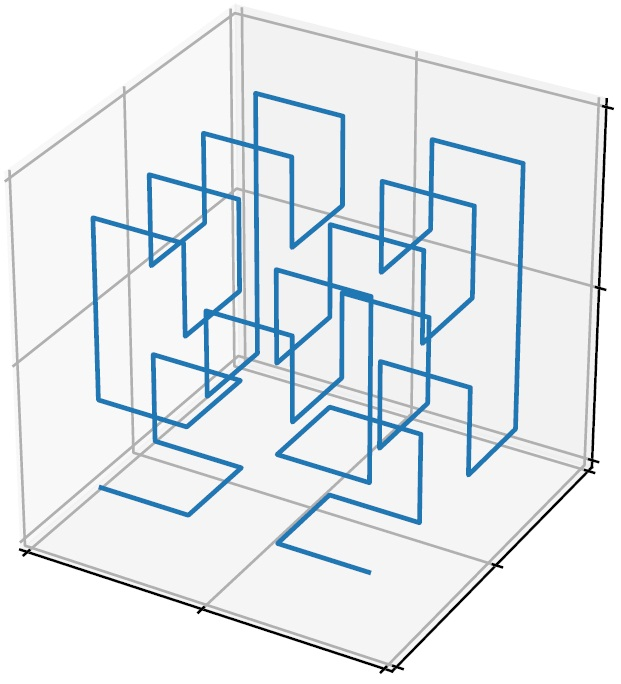
\includegraphics[width=1.0\linewidth]{fig1a.JPG} \\ (a)}
\end{minipage}
\begin{minipage}{0.5\linewidth}
\center{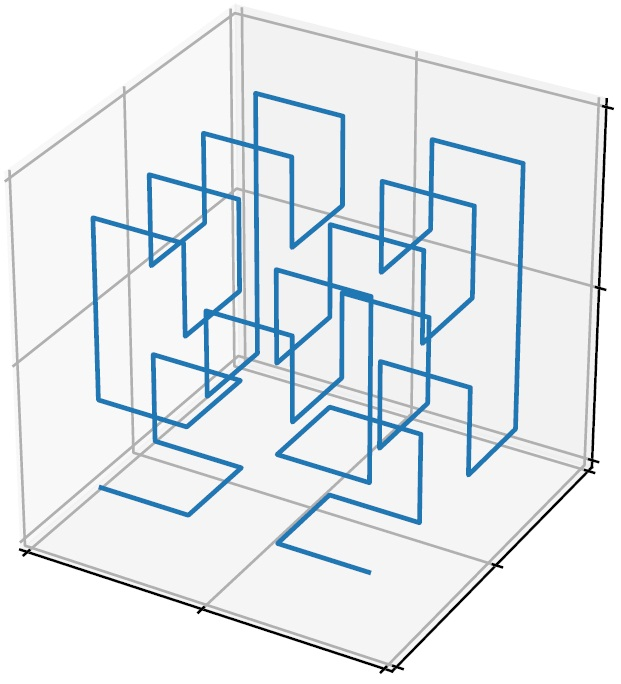
\includegraphics[width=1.0\linewidth]{fig1b.JPG} \\ (b)}
\end{minipage}
\caption{Evolvents in three dimensions with (a) $M=3$ and (b) $M=4$}
\label{evolvents}
\end{figure}


Let us call the process of computing a function value (including the construction of the image $y=y(x)$) as a \textit{trial}, and the pair $\{x, z = \varphi(y(x))\}$ as the outcome of the trial.
When describing a parallel algorithm, we will use the term \textit {iteration} to denote the simultaneous (parallel) execution of several trials (each trial is executed by a separate processor). The number of trials during the $n$-th iteration we will denote as $p$ , and the total number of trials executed during all $n$ iterations as $k(n)$ . In other words, we assume that we have  $p$  processors at our disposal while executing the $n$-th iteration. 

The parallel global search algorithm used in this research (according to \cite{Strongin2000}) can be formulated as follows.
The first $p$ trials are executed at the points $x^0 = 0$, $x^1 = 1$ and at the arbitrary internal points $x^2, ..., x^{p-1}$ of the interval $(0,1)$. Let us assume $n \geq 1$  iterations of the method to be completed, in the course of which the trials in $k=k(n)$ points $x^i, 0 \leq i \leq k,$ have been executed. Then, the points $x^{k+1},...,x^{k+p}$  of the search trials for the next $(n+1)$-th iteration are determined according to the following rules. 

\begin{enumerate}
	\item 
	Renumber the inverse images of all the points from the trials already performed  
\begin{equation}\label{y_i}
y^0=y(x^0), y^1=y(x^1),...,y^k=y(x^k)
\end{equation}
by subscripts in the increasing order of their coordinates, i.e.
\begin{equation}\label{x_i}
0=x_0<x_1<\dots <x_k=1,
\end{equation}
and associate these with the values $z_i=\varphi(y(x_i)), 0\leq i \leq k,$  computed at these points.
\item
Compute the maximum absolute value of the first divided differences
\begin{equation}\label{mu}
\mu = \max_{1 \leq i \leq k}\frac{\left|z_i-z_{i-1}\right|}{\Delta_i},
\end{equation}
where $\Delta_i=\left(x_i-x_{i-1}\right)^{1/N}$. If $\mu = 0$, set $\mu = 1$.
\item
For each interval $(x_{i-1}, x_i), \; 1\leq i \leq k,$  calculate the value
\begin{equation}\label{R}
R(i)=r\mu\Delta_i+\frac{(z_i-z_{i-1})^2}{r\mu\Delta_i}-2(z_i+z_{i-1})
\end{equation}
called the \textit{characteristic} of the interval; the real number $r>1$ being the input parameter of the algorithm.

\item 
Arrange characteristics  $R(i), 1 \leq i \leq k$, in decreasing order 
\begin{equation}\label{Rdec}
R(t_1)\geq R(t_2)\geq \dots \geq R(t_{k})
\end{equation}
and select $p$ largest characteristics with interval numbers $t_j, 1\leq j \leq p$.
\item
Carry out new trials at points $x^{k+j}\in(x_{t_j-1},x_{t_j}), 1\leq j\leq p$, computed according to the formula
\[
x^{k+j} = \frac{x_{t_j}+x_{t_j-1}}{2} - \mathrm{sign}(z_{t_j}-z_{t_j-1})\frac{1}{2r}\left[\frac{\left|z_{t_j}-z_{t_j-1}\right|}{\mu}\right]^N.
\]

\end{enumerate}

The algorithm stops if condition $\Delta_{t_j}<\epsilon$ is satisfied for at least one index $t_j, 1 \leq j \leq p$ ; here $\epsilon>0$ is the predefined accuracy. Also, the algorithm stops if the maximum allowed number of trials $K_{max}$ preset prior to running is exhausted.

%Russian
The considered variant of the parallelization is \textit{synchronous}, when the transition to the next iteration is performed after full termination of the current one, i.e., after completing the last trial of the current iteration.
Particular implementation of this parallelization scheme will depend on the computer system architecture as well as on the requirements to the software necessary for computing the objective function values. In the present study, the conducting of trials required solving a stiff ODE system (for solving this one, Radau IIA method was used). Therefore, the parallelization was organized on CPU using MPI technology. The global search algorithm was run on a single (master) processor. The rest (slave) processors conducted parallel trials within the Step 5 of the algorithm. The amount of data transferred between the processes was small: it was only required to send out the coordinates of trial points and then to collect the computed values of the objective function at these points. At the same time, the time of conducting a single trial was not less 1 sec that considerably exceeded the time of data transfer between the processes. This way, the overhead costs for the data transfer didn't essentially affect the parallelization efficiency.

%Конкретная реализация данной схемы распараллеливания будет зависеть от архитектуры вычислительной системы, а также от требований к программному обеспечению, необходимому для вычисления значений целевой функции задачи. В данном исследовании проведение испытаний требовало решения жесткой системы ODE (для ее решения был использован метод Radau IIA). Поэтому распараллеливание было организовано на CPU с использованием технологии MPI. В одном (master) процессе работал алгоритм глобального поиска; остальные (slave) процессы проводили параллельные испытания в рамках выполнения шага 5 алгоритма. Объем передаваемых данных между процессами был небольшим: требовалось лишь разослать координаты точек испытаний и затем собрать вычисленные значения целевой функции в этих точках. Одновременно с этим время проведения одного испытания составляло не менее 1 сек., что значительно превышает время передачи данных между процессами. Тем самым, накладные расходы на передачу данных не оказывали существенного влияния на эффективность распараллеливания.


\section{Numerical Experiments}\label{Sec_Exp}
%Таким образом, в результате решения обратной задачи химической кинетики параллельным методом глобального поиска были рассчитаны кинетические параметры процесса предриформинга пропана на Ni катализаторе (Table \ref{tab:1}). Для интерпретации полученных результатов проводится решение прямой задачи химической кинетики, то есть расчет концентраций компонентов реакции и сравнение их с экспериментальными данными. На рисунках НОМЕР a, b показано сравнение рассчитанных концентраций с экспериментальными при разных условиях: (a) GHSV 4000 h$^{-1}$, (b) GHSV 12000 h$^{-1}$. Результаты расчетов качественно согласуются с экспериментом. Ошибка отклонения составляет не более ПОСЧИТАТЬ \%.
Thus, as a result of solving the inverse problem of chemical kinetics by the parallel global search method, the kinetic parameters of the propane pre-reforming process on a Ni catalyst were calculated (Table \ref{tab:1}). To interpret the results obtained, the solution of the direct problem of chemical kinetics was carried out, namely, the concentrations of the reaction components were calculated and compared with the experimental data. Fig.~\ref{fig_kin_curves} shows a comparison of the calculated concentrations with the experimental ones under different conditions: (a) GHSV=4000 h$^{-1}$, (b) GHSV=12000 h$^{-1}$. The results of the calculations are qualitatively consistent with the experiment.

\begin{figure}[ht]
	\begin{minipage}{0.5\linewidth}
		\center{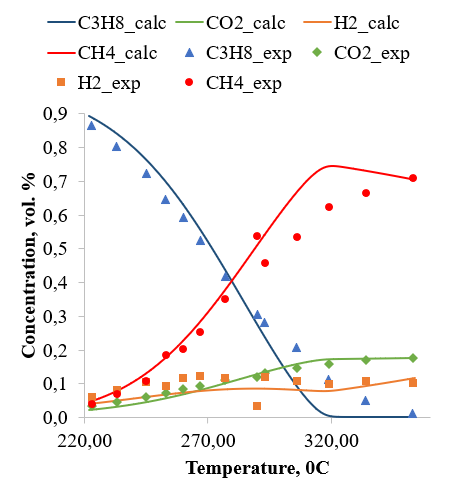
\includegraphics[width=1.0\linewidth]{kin_curve1.png} \\ (a)}
	\end{minipage}
	\begin{minipage}{0.5\linewidth}
		\center{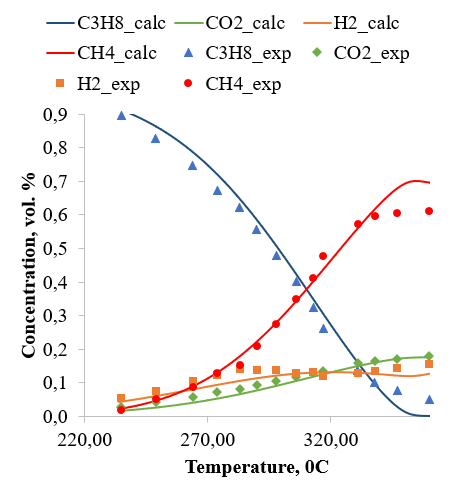
\includegraphics[width=1.0\linewidth]{kin_curve2.png} \\ (b)}
	\end{minipage}
	\caption{Temperature dependences of the output concentrations of propane C3H8, methane CH4, hydrogen H2 and CO2 in the process of propane pre-reforming. Experimental conditions: 220-380 $^0$C, (a) GHSV = 4000 h$^{-1}$, (b) GHSV = 12000 h$^{-1}$, 1 bar pressure. Concentrations of the gas components on the figure are given on the dry basis. Points are experimental concentrations (``exp''-index), lines are simulated concentrations (``calc''-index).}
	\label{fig_kin_curves}
\end{figure}


\begin{table}[ht]
	\caption{Calculated kinetic parameters}
	\label{tab:1}
	\center
	\begin{tabular}{c|c|c|c|c|c}
		\hline
		%\noalign{\smallskip}
		$E_{ref}$, kJ/mol & $E_{met}$, kJ/mol & $k_{ref}$, (mole$\cdot$m$^{-3}$)m$\cdot$s$^{-1}$ & $k_{met}$, s$^{-1}$ & $m$ & $B$ \\
		%\noalign{\smallskip} 
		\hline 
		%\noalign{\smallskip}
		99.23 \;&	37.08 \; & $2.4 \cdot 10^{10}$ \;  & $1.93 \cdot 10^5$ \; & 0.82 & 4.8  \\
		%\noalign{\smallskip}
		\hline
	\end{tabular}
\end{table}
%Для сравнения с предыдущими расчетами был построен график арренисовской зависимости (рисунок НОМЕР), на котором представлены зависимости десятичного логарифма от констант скоростей реакций \eqref{reac_ref} и \eqref{reac_met} от обратной температуры. Обозначения "GA", "GSA" и "PGSA" означают  решения, полученные различными алгоритмами оптимизации, соотвественно, генетическим алгоритмом, алгоритмом гравитационного поиска и параллельным алгоритмом глобального поиска.

For comparison with the previous calculations, an Arrhenis plot was constructed (Fig.~\ref{fig_arren}), which shows the dependence of the decimal logarithm on the reaction rate constants \eqref{reac_ref} and \eqref{reac_met} on the inverse temperature. The designations ``GA'', ``GSA'' and ``PGSA'' mean solutions obtained by various optimization algorithms, the genetic algorithm, the gravity search algorithm, and the parallel global search algorithm, respectively. The blue lines refer to the pre-reforming reaction \eqref{reac_ref}, and the yellow lines refer to the methanation reaction~\eqref{reac_met}. Note that the lines of the same color are parallel to each other, which means that the activation energies of the reaction calculated by different methods have approximately the same values, which indicates the adequacy of the calculations.

\begin{figure}[ht]
	\center{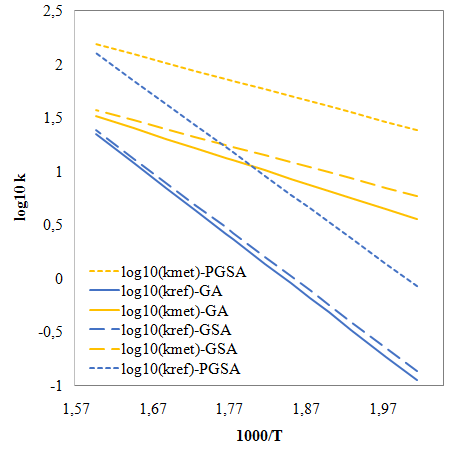
\includegraphics[width=0.8\linewidth]{arren.png}}
	\caption{Comparison of the obtained solution with the other algorithms found on the Arrhenius plot}
	\label{fig_arren}
\end{figure}


Numerical experiments were performed on the Lobachevsky supercomputer of the University of Nizhni Novgorod (operating system -- CentOS 7.2, control system -- SLURM). One supercomputer node has 2 Intel Sandy Bridge E5-2660 2.2 GHz processors, 64 Gb RAM. The CPU is 8-core (i.e. a total of 16 CPU cores are available on the node). The numerical experiments were performed using the Globalizer system \cite{globalizerSystem}.
To build the system for running on the Lobachevsky supercomputer, the GCC 5.5.0 compiler and Intel MPI 2017 were used.
To solve the stiff system of equations arising in computing the objective function values, Radau method from SciPy library from Python 3.9 was used.

%Для решения жесткой системы уравнений, возникающей при вычислении значений целевой функции, использовался метод Radau из библиотеки SciPy, Python 3.9. Global search algorithm запускался со следующими параметрами: параметр надежности $r=5$, точность поиска $\epsilon = 0.01$, плотность построения evolvent $m=10$, максимальное число испытаний $K_{max}=5000$. После завершения работы алгоритма найденное решение уточнялось с помощью локального поиска, использовался Hooke--Jeeves method \cite{HookJeeves}. Точность локального поиска составляла $\epsilon = 0.001$. Для оценки эффективности распараллеливания global search algorithm запускался в последовательном и паралелльном режимах, максимальное число задействованных вычислительных узлов составляло 20, соответственно, максимальное число задействованных процессоров было 40. На Fig.~\ref{fig_time},\ref{fig_speedup} приведены графики, отражающие время и ускорение параллельного алгортима в зависимости от числа процессоров; время работы приведено в часах.


Global search algorithm was run with the following parameters: the reliability parameter $r=5$, the search precision $\epsilon = 0.01$, the evolvent density $m=10$, the maximum allowed number of trials $K_{max}=5000$. Upon completing the execution of the algorithm, the solution found was refined with a local search using Hooke--Jeeves method \cite{HookJeeves}. The local search precision was $\epsilon = 0.001$. 
To evaluate the parallelization efficiency, the global search algorithm was run in the sequential regime and in the parallel one, the maximum number of computer nodes employed was 20. Correspondingly, the maximum number of processors employed was 40.
In Fig.~\ref{fig_time} and Fig.~\ref{fig_speedup} the plots reflecting the running time and the speedup of the parallel algorithm {\em vs} the number of processors employed, respectively are presented (the time is in hours).


\begin{figure}[ht]
\center{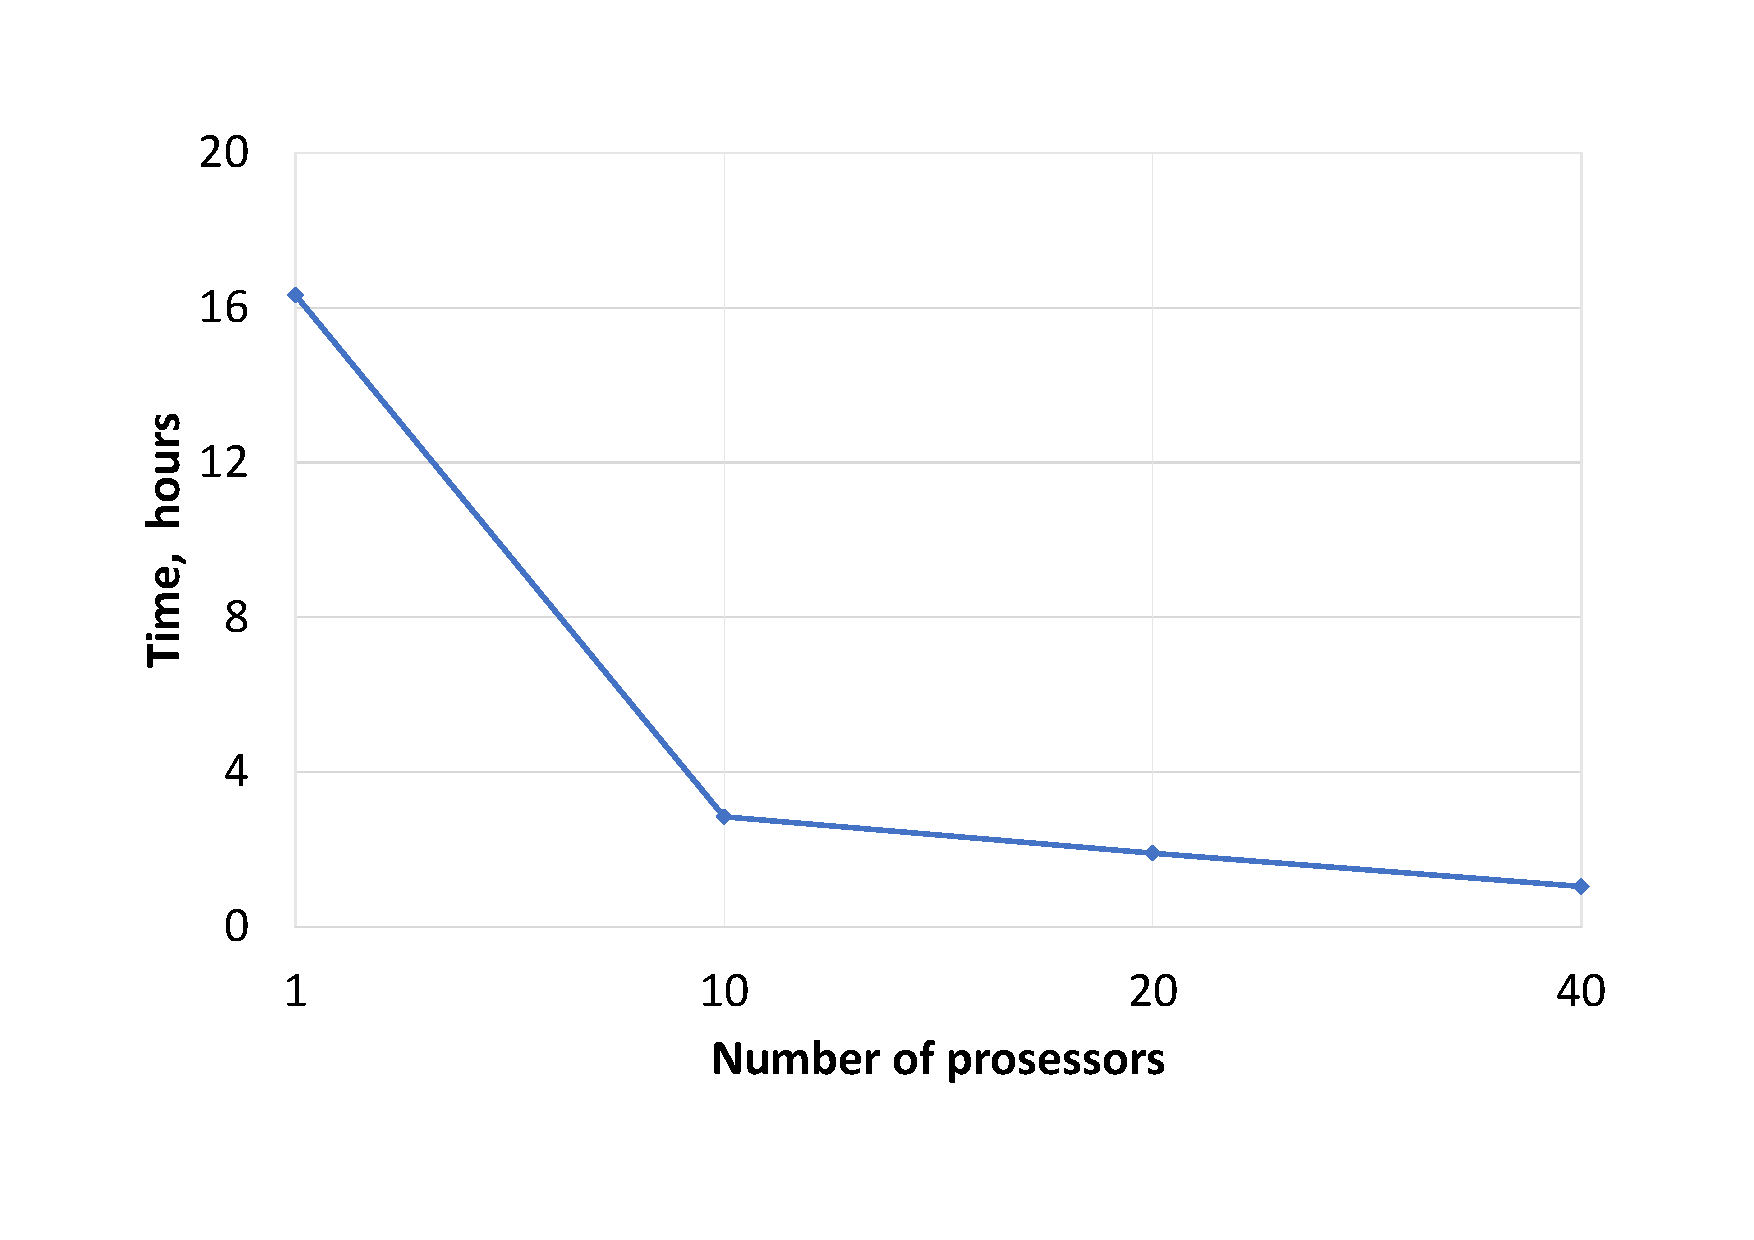
\includegraphics[width=0.8\linewidth]{time.pdf}}
\caption{The parallel algorithm running time}
\label{fig_time}
\end{figure}


\begin{figure}[ht]
\center{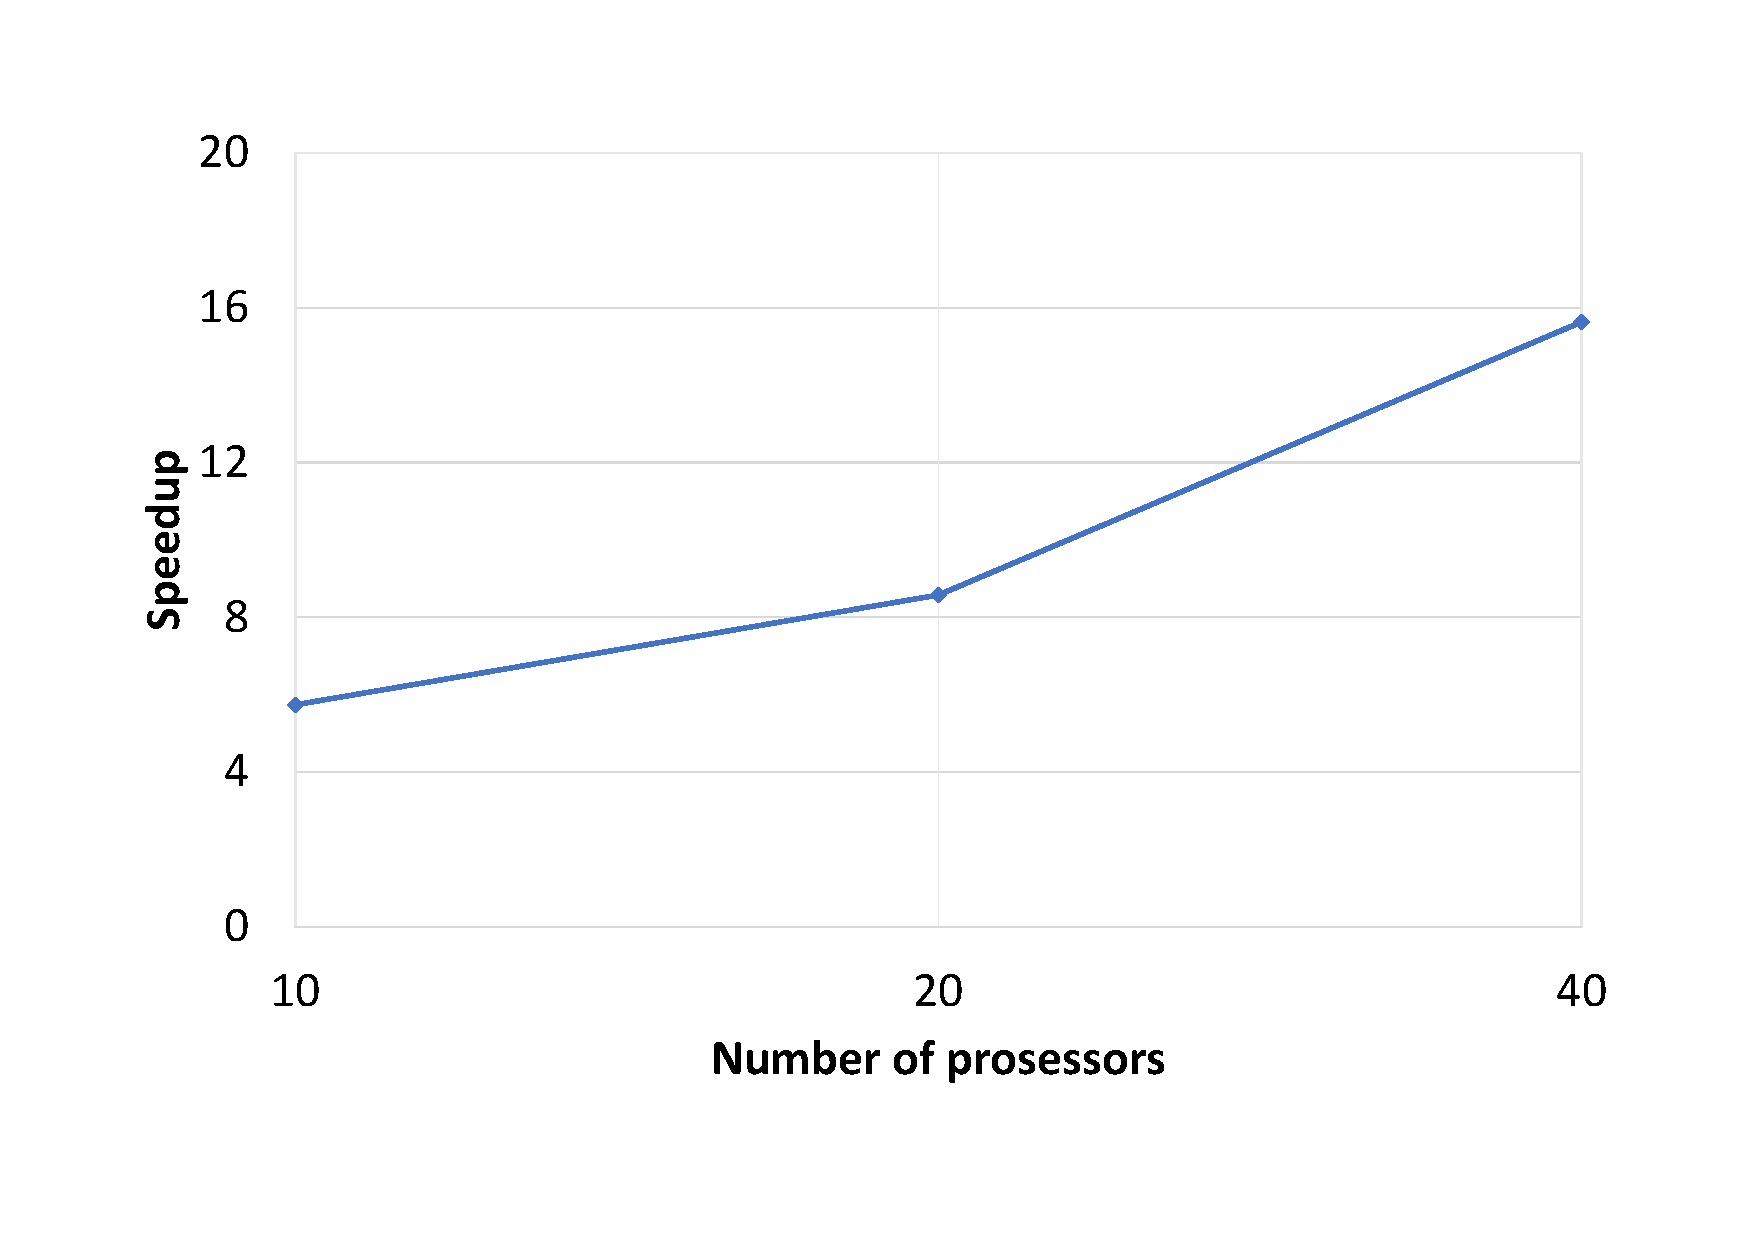
\includegraphics[width=0.8\linewidth]{speedup.pdf}}
\caption{Speedup of the parallel algorithm}
\label{fig_speedup}
\end{figure}




\section{Conclusions and Future Work}

%В будущем планируется моделирование других химических процессов, а именно, первая задача это моделирование процесса сернокислотного алкилирования изобутана олефинами, для которого на данный момент составлена схема химических превращений, проведен литературный обзор процесса и найдены экспериментальные данные. Математическая модель реакции сернокислотного алкилирования изобутана олефинами представляет собой задачу Коши, на данный момент решена прямая задача химической кинетики, далее будет решаться обратная задача предложенными параллельными методами. Вторая задача это моделирование процесса синтеза метил-трет бутилового эфира. Химизм данного процесса известен, задача иемют небольшую размерность, однако моделирование реактора трудоемко и представляет собой решение уравнение в частных производных второго порядка. На данный момент расписана разностная схема, реализован метод прогонки, следующим этапом будет решение прямой задачи химической кинетики, а также предсказание кинетических параметров процесса предложенными параллельными методами.

In the future, it is planned to simulate other chemical processes, namely, the first task is to simulate the process of sulfuric acid alkylation of isobutane with olefins, for which a scheme of chemical transformations has been compiled, a literature review of the process has been conducted, and experimental data have been found. The mathematical model of the reaction of sulfuric acid alkylation of isobutane by olefins is a Cauchy problem, at the moment the direct problem of chemical kinetics is solved, then the inverse problem will be solved by the proposed parallel methods. The second task is to simulate the synthesis of methyl-tert-butyl ether. The chemistry of this process is known, and the problem has a small dimension, but the simulation of the reactor is time-consuming and represents the solution of a second-order partial differential equation. At the moment, the difference scheme is formed, the run-through method is implemented, the next stage will be the solution of the direct problem of chemical kinetics, as well as the prediction of the kinetic parameters of the process by the proposed parallel methods.

%В планы дальнейших работ входит также и повышение эффективности распараллеливания используемого метода. Относительно невысокие показатели ускорения при решении данной задачи объясняются двумя обстоятельствами. Во-первых, при реализации параллельного алгоритма была применена синхронная схема распараллеливания. Управляющий процесс (в котором работал метод оптимизации) при выполнении  шага 5 алгоритма ожидал окончания проведения всех испытаний, проводимых подчиненными процессами. Тогда как в рассматриваемой задаче время проведения одного испытания (как было экспериментально установлено) варьировалось от 1 до 40 секунд в зависимости от конкретных значений параметров. Возможный путь к повышению эффективности распаралелливания - реализация асинхронной схемы проведения испытаний на шаге 5 алгоритма. В этом случае результаты испытания, полученные в одном из подчиненных процессов, могут быть отправлены для обработки в управляющий процесс немедленно, без ожидания окончания других испытаний. После чего подчиненный процесс получает от управляющего процесса новую точку, в которой проводит очередное испытание. Асинхронная схема распараллеливания, теоретически, способна обеспечить полную загрузку задействованных вычислительных ресурсов даже в том случае, когда время выполнения испытаний различно в разных точках области поиска. Во-вторых, при масштабном распараллеливании "узким местом" становится локальный поиск, который выполняется для уточнения решения после завершения фазы глобального поиска. Локальный поиск требует незначительного (по сравнению с глобальным) числа trials, но эти испытания выполняются последовательно. И при паралелльном запуске это незначительное число последовательных испытаний становится сопоставимым с числом параллельных итераций глобального поиска. В дальнейшем планируется использовать параллельную реализацию метода локального поиска на завершающем этапе работы, что способно повысить эффективность распараллеливания в целом.

The plans of further work include also the improvement of the parallelization efficiency for the global optimization method used. Relatively low indicators of speedup in the solving of the present problem can be explained by two factors. First, a synchronous parallelization scheme was applied in the implementation of the parallel algorithm. The master process (which the optimization method worked in) was waiting for the finish of execution of all trials performed by the slave processes when executing Step 5 of the algorithm. However, the time of executing  a single trial in the problem considered varied from 1 up to 40 seconds subject to particular values of parameters (as it was found experimentally). The implementation of the asynchronous scheme of executing the trials at Step 5 of the algorithm seems to be a promising way of improving the parallelization efficiency. 
In this case, the trial results obtained by a slave process may be sent to the master process for processing immediately without waiting for the competing of other trials. Afterwards, the slave process receives a new point of the next trial form the master one. Theoretically, the asynchronous parallelization scheme can provide a full load of the computer resources employed even if the trial execution times are different at different points of the search domain. 

Second, the local search, which is performed to refine the solution after completing the global search phase becomes a ``bottleneck'' at large-scale parallelization. The local search requires insufficient number of trials (as compared to the global one), but these trials should be performed sequentially. And at the parallel run this insufficient number of sequential trials becomes comparable to the number of the parallel global search iterations. 
In future, we plan to use the parallel implementation of the local search method in the final stage of the work that can improve the overall parallelization efficiency.



\medskip

\textbf{Acknowledgments}. This study was supported by the Russian Science Foundation, project No.\,21-11-00204 and by RFBR, project No.\,19-37-60014.

%
% ---- Bibliography ----
%
\bibliographystyle{spmpsci}
\bibliography{bibliography}{}

\end{document}
